\documentclass[twoside]{book}

% Packages required by doxygen
\usepackage{fixltx2e}
\usepackage{calc}
\usepackage{doxygen}
\usepackage{graphicx}
\usepackage[utf8]{inputenc}
\usepackage{makeidx}
\usepackage{multicol}
\usepackage{multirow}
\PassOptionsToPackage{warn}{textcomp}
\usepackage{textcomp}
\usepackage[nointegrals]{wasysym}
\usepackage[table]{xcolor}

% Font selection
\usepackage[T1]{fontenc}
\usepackage{mathptmx}
\usepackage[scaled=.90]{helvet}
\usepackage{courier}
\usepackage{amssymb}
\usepackage{sectsty}
\renewcommand{\familydefault}{\sfdefault}
\allsectionsfont{%
  \fontseries{bc}\selectfont%
  \color{darkgray}%
}
\renewcommand{\DoxyLabelFont}{%
  \fontseries{bc}\selectfont%
  \color{darkgray}%
}
\newcommand{\+}{\discretionary{\mbox{\scriptsize$\hookleftarrow$}}{}{}}

% Page & text layout
\usepackage{geometry}
\geometry{%
  a4paper,%
  top=2.5cm,%
  bottom=2.5cm,%
  left=2.5cm,%
  right=2.5cm%
}
\tolerance=750
\hfuzz=15pt
\hbadness=750
\setlength{\emergencystretch}{15pt}
\setlength{\parindent}{0cm}
\setlength{\parskip}{0.2cm}
\makeatletter
\renewcommand{\paragraph}{%
  \@startsection{paragraph}{4}{0ex}{-1.0ex}{1.0ex}{%
    \normalfont\normalsize\bfseries\SS@parafont%
  }%
}
\renewcommand{\subparagraph}{%
  \@startsection{subparagraph}{5}{0ex}{-1.0ex}{1.0ex}{%
    \normalfont\normalsize\bfseries\SS@subparafont%
  }%
}
\makeatother

% Headers & footers
\usepackage{fancyhdr}
\pagestyle{fancyplain}
\fancyhead[LE]{\fancyplain{}{\bfseries\thepage}}
\fancyhead[CE]{\fancyplain{}{}}
\fancyhead[RE]{\fancyplain{}{\bfseries\leftmark}}
\fancyhead[LO]{\fancyplain{}{\bfseries\rightmark}}
\fancyhead[CO]{\fancyplain{}{}}
\fancyhead[RO]{\fancyplain{}{\bfseries\thepage}}
\fancyfoot[LE]{\fancyplain{}{}}
\fancyfoot[CE]{\fancyplain{}{}}
\fancyfoot[RE]{\fancyplain{}{\bfseries\scriptsize Generated on Mon Oct 31 2016 00\+:04\+:57 for Lab\+C5 by Doxygen }}
\fancyfoot[LO]{\fancyplain{}{\bfseries\scriptsize Generated on Mon Oct 31 2016 00\+:04\+:57 for Lab\+C5 by Doxygen }}
\fancyfoot[CO]{\fancyplain{}{}}
\fancyfoot[RO]{\fancyplain{}{}}
\renewcommand{\footrulewidth}{0.4pt}
\renewcommand{\chaptermark}[1]{%
  \markboth{#1}{}%
}
\renewcommand{\sectionmark}[1]{%
  \markright{\thesection\ #1}%
}

% Indices & bibliography
\usepackage{natbib}
\usepackage[titles]{tocloft}
\setcounter{tocdepth}{3}
\setcounter{secnumdepth}{5}
\makeindex

% Hyperlinks (required, but should be loaded last)
\usepackage{ifpdf}
\ifpdf
  \usepackage[pdftex,pagebackref=true]{hyperref}
\else
  \usepackage[ps2pdf,pagebackref=true]{hyperref}
\fi
\hypersetup{%
  colorlinks=true,%
  linkcolor=blue,%
  citecolor=blue,%
  unicode%
}

% Custom commands
\newcommand{\clearemptydoublepage}{%
  \newpage{\pagestyle{empty}\cleardoublepage}%
}


%===== C O N T E N T S =====

\begin{document}

% Titlepage & ToC
\hypersetup{pageanchor=false,
             bookmarks=true,
             bookmarksnumbered=true,
             pdfencoding=unicode
            }
\pagenumbering{roman}
\begin{titlepage}
\vspace*{7cm}
\begin{center}%
{\Large Lab\+C5 \\[1ex]\large 1.\+0 }\\
\vspace*{1cm}
{\large Generated by Doxygen 1.8.8}\\
\vspace*{0.5cm}
{\small Mon Oct 31 2016 00:04:57}\\
\end{center}
\end{titlepage}
\clearemptydoublepage
\tableofcontents
\clearemptydoublepage
\pagenumbering{arabic}
\hypersetup{pageanchor=true}

%--- Begin generated contents ---
\chapter{Class Index}
\section{Class List}
Here are the classes, structs, unions and interfaces with brief descriptions\+:\begin{DoxyCompactList}
\item\contentsline{section}{\hyperlink{class_calculadora}{Calculadora$<$ data $>$} }{\pageref{class_calculadora}}{}
\item\contentsline{section}{\hyperlink{class_fraccion}{Fraccion} }{\pageref{class_fraccion}}{}
\item\contentsline{section}{\hyperlink{class_matriz}{Matriz} }{\pageref{class_matriz}}{}
\item\contentsline{section}{\hyperlink{class_polinomio}{Polinomio} }{\pageref{class_polinomio}}{}
\end{DoxyCompactList}

\chapter{File Index}
\section{File List}
Here is a list of all files with brief descriptions\+:\begin{DoxyCompactList}
\item\contentsline{section}{\hyperlink{_circulo_8cpp}{Circulo.\+cpp} }{\pageref{_circulo_8cpp}}{}
\item\contentsline{section}{\hyperlink{_circulo_8h}{Circulo.\+h} }{\pageref{_circulo_8h}}{}
\item\contentsline{section}{\hyperlink{_cuadrado_8cpp}{Cuadrado.\+cpp} }{\pageref{_cuadrado_8cpp}}{}
\item\contentsline{section}{\hyperlink{_cuadrado_8h}{Cuadrado.\+h} }{\pageref{_cuadrado_8h}}{}
\item\contentsline{section}{\hyperlink{_figura_8cpp}{Figura.\+cpp} }{\pageref{_figura_8cpp}}{}
\item\contentsline{section}{\hyperlink{_figura_8h}{Figura.\+h} }{\pageref{_figura_8h}}{}
\item\contentsline{section}{\hyperlink{main_8cpp}{main.\+cpp} }{\pageref{main_8cpp}}{}
\item\contentsline{section}{\hyperlink{_triangulo_8cpp}{Triangulo.\+cpp} }{\pageref{_triangulo_8cpp}}{}
\item\contentsline{section}{\hyperlink{_triangulo_8h}{Triangulo.\+h} }{\pageref{_triangulo_8h}}{}
\end{DoxyCompactList}

\chapter{Class Documentation}
\hypertarget{class_carta}{\section{Carta Class Reference}
\label{class_carta}\index{Carta@{Carta}}
}


{\ttfamily \#include $<$Carta.\+h$>$}



Collaboration diagram for Carta\+:
\nopagebreak
\begin{figure}[H]
\begin{center}
\leavevmode
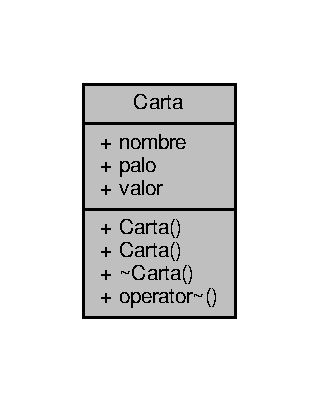
\includegraphics[width=153pt]{class_carta__coll__graph}
\end{center}
\end{figure}
\subsection*{Public Member Functions}
\begin{DoxyCompactItemize}
\item 
\hyperlink{class_carta_a769e6bdb8d3725177481b32e4dbbbd66}{Carta} ()
\begin{DoxyCompactList}\small\item\em Constructor básico de la clase \hyperlink{class_carta}{Carta}. \end{DoxyCompactList}\item 
\hyperlink{class_carta_a0801c30475b4d0331e42e29b96300142}{Carta} (string \hyperlink{class_carta_af9ecddff3f4ac2ffe4a00a5ec62a3b29}{nombre}, string \hyperlink{class_carta_a708b56ce311c1ea2329a76c60d740881}{palo}, int \hyperlink{class_carta_a40ed698935c3b770a0b118dea14c667b}{valor})
\begin{DoxyCompactList}\small\item\em Constructor con características de la clase \hyperlink{class_carta}{Carta}. \end{DoxyCompactList}\item 
\hyperlink{class_carta_ae3f30ed1ac1712b56330186f9e2139ec}{$\sim$\+Carta} ()
\begin{DoxyCompactList}\small\item\em Destructor de la clase \hyperlink{class_carta}{Carta}. \end{DoxyCompactList}\item 
void \hyperlink{class_carta_a0e5b4b65152cb3a1147c1dcb019f7def}{operator$\sim$} ()
\begin{DoxyCompactList}\small\item\em Método de print para la clase \hyperlink{class_carta}{Carta}. \end{DoxyCompactList}\end{DoxyCompactItemize}
\subsection*{Public Attributes}
\begin{DoxyCompactItemize}
\item 
string \hyperlink{class_carta_af9ecddff3f4ac2ffe4a00a5ec62a3b29}{nombre}
\item 
string \hyperlink{class_carta_a708b56ce311c1ea2329a76c60d740881}{palo}
\item 
int \hyperlink{class_carta_a40ed698935c3b770a0b118dea14c667b}{valor}
\end{DoxyCompactItemize}


\subsection{Constructor \& Destructor Documentation}
\hypertarget{class_carta_a769e6bdb8d3725177481b32e4dbbbd66}{\index{Carta@{Carta}!Carta@{Carta}}
\index{Carta@{Carta}!Carta@{Carta}}
\subsubsection[{Carta}]{\setlength{\rightskip}{0pt plus 5cm}Carta\+::\+Carta (
\begin{DoxyParamCaption}
{}
\end{DoxyParamCaption}
)}}\label{class_carta_a769e6bdb8d3725177481b32e4dbbbd66}


Constructor básico de la clase \hyperlink{class_carta}{Carta}. 

\hypertarget{class_carta_a0801c30475b4d0331e42e29b96300142}{\index{Carta@{Carta}!Carta@{Carta}}
\index{Carta@{Carta}!Carta@{Carta}}
\subsubsection[{Carta}]{\setlength{\rightskip}{0pt plus 5cm}Carta\+::\+Carta (
\begin{DoxyParamCaption}
\item[{string}]{nombre, }
\item[{string}]{palo, }
\item[{int}]{valor}
\end{DoxyParamCaption}
)}}\label{class_carta_a0801c30475b4d0331e42e29b96300142}


Constructor con características de la clase \hyperlink{class_carta}{Carta}. 

\hypertarget{class_carta_ae3f30ed1ac1712b56330186f9e2139ec}{\index{Carta@{Carta}!````~Carta@{$\sim$\+Carta}}
\index{````~Carta@{$\sim$\+Carta}!Carta@{Carta}}
\subsubsection[{$\sim$\+Carta}]{\setlength{\rightskip}{0pt plus 5cm}Carta\+::$\sim$\+Carta (
\begin{DoxyParamCaption}
{}
\end{DoxyParamCaption}
)}}\label{class_carta_ae3f30ed1ac1712b56330186f9e2139ec}


Destructor de la clase \hyperlink{class_carta}{Carta}. 



\subsection{Member Function Documentation}
\hypertarget{class_carta_a0e5b4b65152cb3a1147c1dcb019f7def}{\index{Carta@{Carta}!operator````~@{operator$\sim$}}
\index{operator````~@{operator$\sim$}!Carta@{Carta}}
\subsubsection[{operator$\sim$}]{\setlength{\rightskip}{0pt plus 5cm}void Carta\+::operator$\sim$ (
\begin{DoxyParamCaption}
{}
\end{DoxyParamCaption}
)}}\label{class_carta_a0e5b4b65152cb3a1147c1dcb019f7def}


Método de print para la clase \hyperlink{class_carta}{Carta}. 



\subsection{Member Data Documentation}
\hypertarget{class_carta_af9ecddff3f4ac2ffe4a00a5ec62a3b29}{\index{Carta@{Carta}!nombre@{nombre}}
\index{nombre@{nombre}!Carta@{Carta}}
\subsubsection[{nombre}]{\setlength{\rightskip}{0pt plus 5cm}string Carta\+::nombre}}\label{class_carta_af9ecddff3f4ac2ffe4a00a5ec62a3b29}
\hypertarget{class_carta_a708b56ce311c1ea2329a76c60d740881}{\index{Carta@{Carta}!palo@{palo}}
\index{palo@{palo}!Carta@{Carta}}
\subsubsection[{palo}]{\setlength{\rightskip}{0pt plus 5cm}string Carta\+::palo}}\label{class_carta_a708b56ce311c1ea2329a76c60d740881}
\hypertarget{class_carta_a40ed698935c3b770a0b118dea14c667b}{\index{Carta@{Carta}!valor@{valor}}
\index{valor@{valor}!Carta@{Carta}}
\subsubsection[{valor}]{\setlength{\rightskip}{0pt plus 5cm}int Carta\+::valor}}\label{class_carta_a40ed698935c3b770a0b118dea14c667b}


The documentation for this class was generated from the following files\+:\begin{DoxyCompactItemize}
\item 
/home/emanuel/\+Desktop/\+Labs/\+Lab\+C5/src/\hyperlink{_carta_8h}{Carta.\+h}\item 
/home/emanuel/\+Desktop/\+Labs/\+Lab\+C5/src/\hyperlink{_carta_8cpp}{Carta.\+cpp}\end{DoxyCompactItemize}

\hypertarget{class_fila}{\section{Fila Class Reference}
\label{class_fila}\index{Fila@{Fila}}
}


{\ttfamily \#include $<$Fila.\+h$>$}



Collaboration diagram for Fila\+:
\nopagebreak
\begin{figure}[H]
\begin{center}
\leavevmode
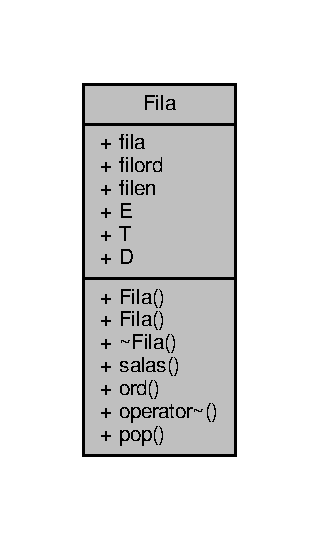
\includegraphics[width=153pt]{class_fila__coll__graph}
\end{center}
\end{figure}
\subsection*{Public Member Functions}
\begin{DoxyCompactItemize}
\item 
\hyperlink{class_fila_ad758c612ef929ffb32cdceb442a5e6a5}{Fila} ()
\begin{DoxyCompactList}\small\item\em Constructor básico de la clase \hyperlink{class_fila}{Fila}. \end{DoxyCompactList}\item 
\hyperlink{class_fila_a2b120e186a1e620ee2c6bacf2c0ea44c}{Fila} (char $\ast$\hyperlink{class_fila_a36a3d7e1492ea5bc367a23f6af9d1ce7}{fila})
\begin{DoxyCompactList}\small\item\em Constructor con características de la clase \hyperlink{class_fila}{Fila}. \end{DoxyCompactList}\item 
\hyperlink{class_fila_af747f8a50e93b382c78e0576a5b40426}{$\sim$\+Fila} ()
\begin{DoxyCompactList}\small\item\em Destructor de la clase \hyperlink{class_fila}{Fila}. \end{DoxyCompactList}\item 
void \hyperlink{class_fila_a1b4a951498a56359211cc3334050c362}{salas} ()
\begin{DoxyCompactList}\small\item\em Método de la clase fila que crea salas de espera en las cuales agrupa a su contenido según su tipo. \end{DoxyCompactList}\item 
void \hyperlink{class_fila_a37535ed9d5d95be4c8c06f216818f7bd}{ord} ()
\begin{DoxyCompactList}\small\item\em Método que ordena la fila según la prioridad. \end{DoxyCompactList}\item 
void \hyperlink{class_fila_a329402e2861273f0b15c23a080a7ff3b}{operator$\sim$} ()
\begin{DoxyCompactList}\small\item\em Método de impresión para la clase \hyperlink{class_fila}{Fila}. \end{DoxyCompactList}\item 
char \hyperlink{class_fila_a56d36d67fb631d3a1ec48bf3b6e55e40}{pop} (bool cond)
\begin{DoxyCompactList}\small\item\em Método que extrae el último elemento de la cola fila ordenada. \end{DoxyCompactList}\end{DoxyCompactItemize}
\subsection*{Public Attributes}
\begin{DoxyCompactItemize}
\item 
char $\ast$ \hyperlink{class_fila_a36a3d7e1492ea5bc367a23f6af9d1ce7}{fila}
\item 
char $\ast$ \hyperlink{class_fila_ae89d6f3b865cf2e4fb66cb793df4b9d6}{filord}
\item 
int \hyperlink{class_fila_a8da3061b2ff7c7a9c93571383c345294}{filen}
\item 
int \hyperlink{class_fila_a8c0087eed7062cb6646d380727e1f8ad}{E}
\item 
int \hyperlink{class_fila_aa22383da45e0e0292cc7d137af754812}{T}
\item 
int \hyperlink{class_fila_aee0859c7d7a52dc7436f7ff899ee0e58}{D}
\end{DoxyCompactItemize}


\subsection{Constructor \& Destructor Documentation}
\hypertarget{class_fila_ad758c612ef929ffb32cdceb442a5e6a5}{\index{Fila@{Fila}!Fila@{Fila}}
\index{Fila@{Fila}!Fila@{Fila}}
\subsubsection[{Fila}]{\setlength{\rightskip}{0pt plus 5cm}Fila\+::\+Fila (
\begin{DoxyParamCaption}
{}
\end{DoxyParamCaption}
)}}\label{class_fila_ad758c612ef929ffb32cdceb442a5e6a5}


Constructor básico de la clase \hyperlink{class_fila}{Fila}. 

\hypertarget{class_fila_a2b120e186a1e620ee2c6bacf2c0ea44c}{\index{Fila@{Fila}!Fila@{Fila}}
\index{Fila@{Fila}!Fila@{Fila}}
\subsubsection[{Fila}]{\setlength{\rightskip}{0pt plus 5cm}Fila\+::\+Fila (
\begin{DoxyParamCaption}
\item[{char $\ast$}]{fila}
\end{DoxyParamCaption}
)}}\label{class_fila_a2b120e186a1e620ee2c6bacf2c0ea44c}


Constructor con características de la clase \hyperlink{class_fila}{Fila}. 

\hypertarget{class_fila_af747f8a50e93b382c78e0576a5b40426}{\index{Fila@{Fila}!````~Fila@{$\sim$\+Fila}}
\index{````~Fila@{$\sim$\+Fila}!Fila@{Fila}}
\subsubsection[{$\sim$\+Fila}]{\setlength{\rightskip}{0pt plus 5cm}Fila\+::$\sim$\+Fila (
\begin{DoxyParamCaption}
{}
\end{DoxyParamCaption}
)}}\label{class_fila_af747f8a50e93b382c78e0576a5b40426}


Destructor de la clase \hyperlink{class_fila}{Fila}. 



\subsection{Member Function Documentation}
\hypertarget{class_fila_a329402e2861273f0b15c23a080a7ff3b}{\index{Fila@{Fila}!operator````~@{operator$\sim$}}
\index{operator````~@{operator$\sim$}!Fila@{Fila}}
\subsubsection[{operator$\sim$}]{\setlength{\rightskip}{0pt plus 5cm}void Fila\+::operator$\sim$ (
\begin{DoxyParamCaption}
{}
\end{DoxyParamCaption}
)}}\label{class_fila_a329402e2861273f0b15c23a080a7ff3b}


Método de impresión para la clase \hyperlink{class_fila}{Fila}. 

\hypertarget{class_fila_a37535ed9d5d95be4c8c06f216818f7bd}{\index{Fila@{Fila}!ord@{ord}}
\index{ord@{ord}!Fila@{Fila}}
\subsubsection[{ord}]{\setlength{\rightskip}{0pt plus 5cm}void Fila\+::ord (
\begin{DoxyParamCaption}
{}
\end{DoxyParamCaption}
)}}\label{class_fila_a37535ed9d5d95be4c8c06f216818f7bd}


Método que ordena la fila según la prioridad. 



Here is the call graph for this function\+:
\nopagebreak
\begin{figure}[H]
\begin{center}
\leavevmode
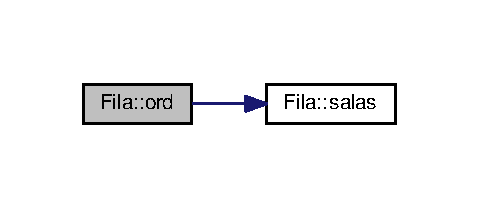
\includegraphics[width=230pt]{class_fila_a37535ed9d5d95be4c8c06f216818f7bd_cgraph}
\end{center}
\end{figure}




Here is the caller graph for this function\+:
\nopagebreak
\begin{figure}[H]
\begin{center}
\leavevmode
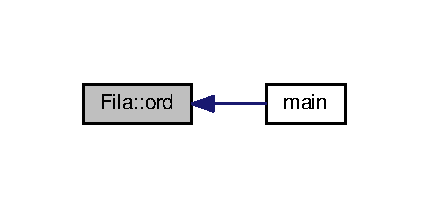
\includegraphics[width=206pt]{class_fila_a37535ed9d5d95be4c8c06f216818f7bd_icgraph}
\end{center}
\end{figure}


\hypertarget{class_fila_a56d36d67fb631d3a1ec48bf3b6e55e40}{\index{Fila@{Fila}!pop@{pop}}
\index{pop@{pop}!Fila@{Fila}}
\subsubsection[{pop}]{\setlength{\rightskip}{0pt plus 5cm}char Fila\+::pop (
\begin{DoxyParamCaption}
\item[{bool}]{cond}
\end{DoxyParamCaption}
)}}\label{class_fila_a56d36d67fb631d3a1ec48bf3b6e55e40}


Método que extrae el último elemento de la cola fila ordenada. 



Here is the caller graph for this function\+:
\nopagebreak
\begin{figure}[H]
\begin{center}
\leavevmode
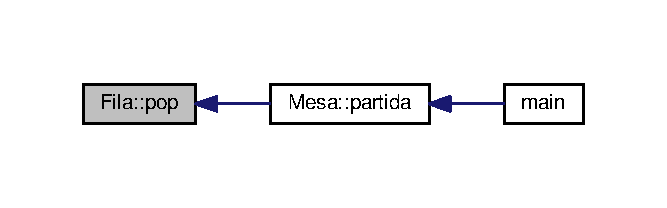
\includegraphics[width=320pt]{class_fila_a56d36d67fb631d3a1ec48bf3b6e55e40_icgraph}
\end{center}
\end{figure}


\hypertarget{class_fila_a1b4a951498a56359211cc3334050c362}{\index{Fila@{Fila}!salas@{salas}}
\index{salas@{salas}!Fila@{Fila}}
\subsubsection[{salas}]{\setlength{\rightskip}{0pt plus 5cm}void Fila\+::salas (
\begin{DoxyParamCaption}
{}
\end{DoxyParamCaption}
)}}\label{class_fila_a1b4a951498a56359211cc3334050c362}


Método de la clase fila que crea salas de espera en las cuales agrupa a su contenido según su tipo. 



Here is the caller graph for this function\+:
\nopagebreak
\begin{figure}[H]
\begin{center}
\leavevmode
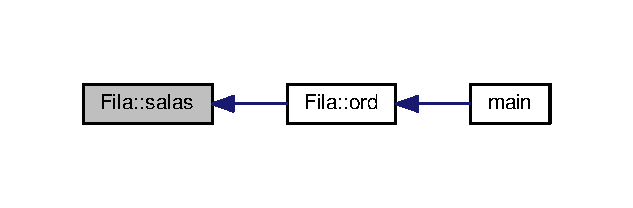
\includegraphics[width=304pt]{class_fila_a1b4a951498a56359211cc3334050c362_icgraph}
\end{center}
\end{figure}




\subsection{Member Data Documentation}
\hypertarget{class_fila_aee0859c7d7a52dc7436f7ff899ee0e58}{\index{Fila@{Fila}!D@{D}}
\index{D@{D}!Fila@{Fila}}
\subsubsection[{D}]{\setlength{\rightskip}{0pt plus 5cm}int Fila\+::\+D}}\label{class_fila_aee0859c7d7a52dc7436f7ff899ee0e58}
\hypertarget{class_fila_a8c0087eed7062cb6646d380727e1f8ad}{\index{Fila@{Fila}!E@{E}}
\index{E@{E}!Fila@{Fila}}
\subsubsection[{E}]{\setlength{\rightskip}{0pt plus 5cm}int Fila\+::\+E}}\label{class_fila_a8c0087eed7062cb6646d380727e1f8ad}
\hypertarget{class_fila_a36a3d7e1492ea5bc367a23f6af9d1ce7}{\index{Fila@{Fila}!fila@{fila}}
\index{fila@{fila}!Fila@{Fila}}
\subsubsection[{fila}]{\setlength{\rightskip}{0pt plus 5cm}char$\ast$ Fila\+::fila}}\label{class_fila_a36a3d7e1492ea5bc367a23f6af9d1ce7}
\hypertarget{class_fila_a8da3061b2ff7c7a9c93571383c345294}{\index{Fila@{Fila}!filen@{filen}}
\index{filen@{filen}!Fila@{Fila}}
\subsubsection[{filen}]{\setlength{\rightskip}{0pt plus 5cm}int Fila\+::filen}}\label{class_fila_a8da3061b2ff7c7a9c93571383c345294}
\hypertarget{class_fila_ae89d6f3b865cf2e4fb66cb793df4b9d6}{\index{Fila@{Fila}!filord@{filord}}
\index{filord@{filord}!Fila@{Fila}}
\subsubsection[{filord}]{\setlength{\rightskip}{0pt plus 5cm}char$\ast$ Fila\+::filord}}\label{class_fila_ae89d6f3b865cf2e4fb66cb793df4b9d6}
\hypertarget{class_fila_aa22383da45e0e0292cc7d137af754812}{\index{Fila@{Fila}!T@{T}}
\index{T@{T}!Fila@{Fila}}
\subsubsection[{T}]{\setlength{\rightskip}{0pt plus 5cm}int Fila\+::\+T}}\label{class_fila_aa22383da45e0e0292cc7d137af754812}


The documentation for this class was generated from the following files\+:\begin{DoxyCompactItemize}
\item 
/home/emanuel/\+Desktop/\+Labs/\+Lab\+C5/src/\hyperlink{_fila_8h}{Fila.\+h}\item 
/home/emanuel/\+Desktop/\+Labs/\+Lab\+C5/src/\hyperlink{_fila_8cpp}{Fila.\+cpp}\end{DoxyCompactItemize}

\hypertarget{class_jugador}{\section{Jugador Class Reference}
\label{class_jugador}\index{Jugador@{Jugador}}
}


{\ttfamily \#include $<$Jugador.\+h$>$}



Collaboration diagram for Jugador\+:
\nopagebreak
\begin{figure}[H]
\begin{center}
\leavevmode
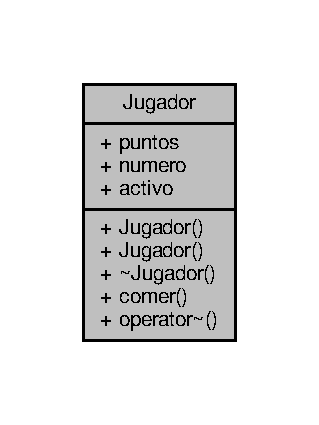
\includegraphics[width=153pt]{class_jugador__coll__graph}
\end{center}
\end{figure}
\subsection*{Public Member Functions}
\begin{DoxyCompactItemize}
\item 
\hyperlink{class_jugador_a232c46f75691af6210096e5972535d71}{Jugador} ()
\begin{DoxyCompactList}\small\item\em Constructor básico de la clase \hyperlink{class_jugador}{Jugador}. \end{DoxyCompactList}\item 
\hyperlink{class_jugador_a7a2ed7131d027122be6eb89baf919bc9}{Jugador} (int n)
\begin{DoxyCompactList}\small\item\em Constructor con características de la clase \hyperlink{class_jugador}{Jugador}. \end{DoxyCompactList}\item 
\hyperlink{class_jugador_a9db1d422fe3b675f92d9fd687b1f42c4}{$\sim$\+Jugador} ()
\begin{DoxyCompactList}\small\item\em Destructor de la clase \hyperlink{class_jugador}{Jugador}. \end{DoxyCompactList}\item 
void \hyperlink{class_jugador_a08b73142c7216db984dede56ccb15d1a}{comer} (\hyperlink{class_mazo}{Mazo} \&mazo)
\begin{DoxyCompactList}\small\item\em Método de la clase jugador para comer carta de un mazo. \end{DoxyCompactList}\item 
void \hyperlink{class_jugador_a74982f759e1f8fcbbd9b8182f03665df}{operator$\sim$} ()
\begin{DoxyCompactList}\small\item\em Método de print para objetos \hyperlink{class_jugador}{Jugador}. \end{DoxyCompactList}\end{DoxyCompactItemize}
\subsection*{Public Attributes}
\begin{DoxyCompactItemize}
\item 
int \hyperlink{class_jugador_a4e264d857d5a3f1a68cbb13e4b88930f}{puntos}
\item 
int \hyperlink{class_jugador_a974067cd6559949ff6b186d53bf4b420}{numero}
\item 
bool \hyperlink{class_jugador_a71f25f6ca8126364057d932d556b533e}{activo}
\end{DoxyCompactItemize}


\subsection{Constructor \& Destructor Documentation}
\hypertarget{class_jugador_a232c46f75691af6210096e5972535d71}{\index{Jugador@{Jugador}!Jugador@{Jugador}}
\index{Jugador@{Jugador}!Jugador@{Jugador}}
\subsubsection[{Jugador}]{\setlength{\rightskip}{0pt plus 5cm}Jugador\+::\+Jugador (
\begin{DoxyParamCaption}
{}
\end{DoxyParamCaption}
)}}\label{class_jugador_a232c46f75691af6210096e5972535d71}


Constructor básico de la clase \hyperlink{class_jugador}{Jugador}. 

\hypertarget{class_jugador_a7a2ed7131d027122be6eb89baf919bc9}{\index{Jugador@{Jugador}!Jugador@{Jugador}}
\index{Jugador@{Jugador}!Jugador@{Jugador}}
\subsubsection[{Jugador}]{\setlength{\rightskip}{0pt plus 5cm}Jugador\+::\+Jugador (
\begin{DoxyParamCaption}
\item[{int}]{n}
\end{DoxyParamCaption}
)}}\label{class_jugador_a7a2ed7131d027122be6eb89baf919bc9}


Constructor con características de la clase \hyperlink{class_jugador}{Jugador}. 

\hypertarget{class_jugador_a9db1d422fe3b675f92d9fd687b1f42c4}{\index{Jugador@{Jugador}!````~Jugador@{$\sim$\+Jugador}}
\index{````~Jugador@{$\sim$\+Jugador}!Jugador@{Jugador}}
\subsubsection[{$\sim$\+Jugador}]{\setlength{\rightskip}{0pt plus 5cm}Jugador\+::$\sim$\+Jugador (
\begin{DoxyParamCaption}
{}
\end{DoxyParamCaption}
)}}\label{class_jugador_a9db1d422fe3b675f92d9fd687b1f42c4}


Destructor de la clase \hyperlink{class_jugador}{Jugador}. 



\subsection{Member Function Documentation}
\hypertarget{class_jugador_a08b73142c7216db984dede56ccb15d1a}{\index{Jugador@{Jugador}!comer@{comer}}
\index{comer@{comer}!Jugador@{Jugador}}
\subsubsection[{comer}]{\setlength{\rightskip}{0pt plus 5cm}void Jugador\+::comer (
\begin{DoxyParamCaption}
\item[{{\bf Mazo} \&}]{mazo}
\end{DoxyParamCaption}
)}}\label{class_jugador_a08b73142c7216db984dede56ccb15d1a}


Método de la clase jugador para comer carta de un mazo. 



Here is the call graph for this function\+:
\nopagebreak
\begin{figure}[H]
\begin{center}
\leavevmode
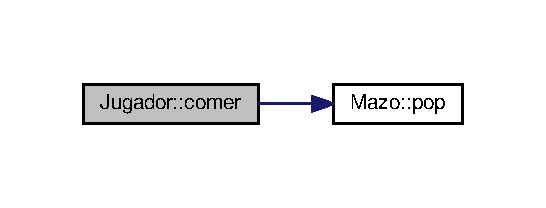
\includegraphics[width=262pt]{class_jugador_a08b73142c7216db984dede56ccb15d1a_cgraph}
\end{center}
\end{figure}




Here is the caller graph for this function\+:
\nopagebreak
\begin{figure}[H]
\begin{center}
\leavevmode
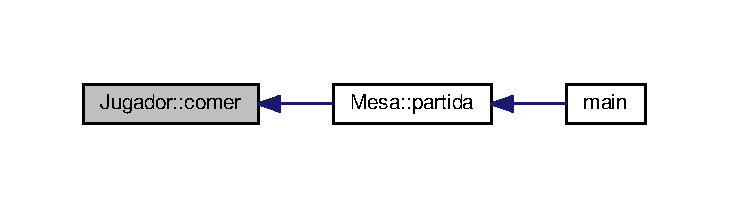
\includegraphics[width=350pt]{class_jugador_a08b73142c7216db984dede56ccb15d1a_icgraph}
\end{center}
\end{figure}


\hypertarget{class_jugador_a74982f759e1f8fcbbd9b8182f03665df}{\index{Jugador@{Jugador}!operator````~@{operator$\sim$}}
\index{operator````~@{operator$\sim$}!Jugador@{Jugador}}
\subsubsection[{operator$\sim$}]{\setlength{\rightskip}{0pt plus 5cm}void Jugador\+::operator$\sim$ (
\begin{DoxyParamCaption}
{}
\end{DoxyParamCaption}
)}}\label{class_jugador_a74982f759e1f8fcbbd9b8182f03665df}


Método de print para objetos \hyperlink{class_jugador}{Jugador}. 



\subsection{Member Data Documentation}
\hypertarget{class_jugador_a71f25f6ca8126364057d932d556b533e}{\index{Jugador@{Jugador}!activo@{activo}}
\index{activo@{activo}!Jugador@{Jugador}}
\subsubsection[{activo}]{\setlength{\rightskip}{0pt plus 5cm}bool Jugador\+::activo}}\label{class_jugador_a71f25f6ca8126364057d932d556b533e}
\hypertarget{class_jugador_a974067cd6559949ff6b186d53bf4b420}{\index{Jugador@{Jugador}!numero@{numero}}
\index{numero@{numero}!Jugador@{Jugador}}
\subsubsection[{numero}]{\setlength{\rightskip}{0pt plus 5cm}int Jugador\+::numero}}\label{class_jugador_a974067cd6559949ff6b186d53bf4b420}
\hypertarget{class_jugador_a4e264d857d5a3f1a68cbb13e4b88930f}{\index{Jugador@{Jugador}!puntos@{puntos}}
\index{puntos@{puntos}!Jugador@{Jugador}}
\subsubsection[{puntos}]{\setlength{\rightskip}{0pt plus 5cm}int Jugador\+::puntos}}\label{class_jugador_a4e264d857d5a3f1a68cbb13e4b88930f}


The documentation for this class was generated from the following files\+:\begin{DoxyCompactItemize}
\item 
/home/emanuel/\+Desktop/\+Labs/\+Lab\+C5/src/\hyperlink{_jugador_8h}{Jugador.\+h}\item 
/home/emanuel/\+Desktop/\+Labs/\+Lab\+C5/src/\hyperlink{_jugador_8cpp}{Jugador.\+cpp}\end{DoxyCompactItemize}

\hypertarget{class_mazo}{\section{Mazo Class Reference}
\label{class_mazo}\index{Mazo@{Mazo}}
}


{\ttfamily \#include $<$Mazo.\+h$>$}



Collaboration diagram for Mazo\+:
\nopagebreak
\begin{figure}[H]
\begin{center}
\leavevmode
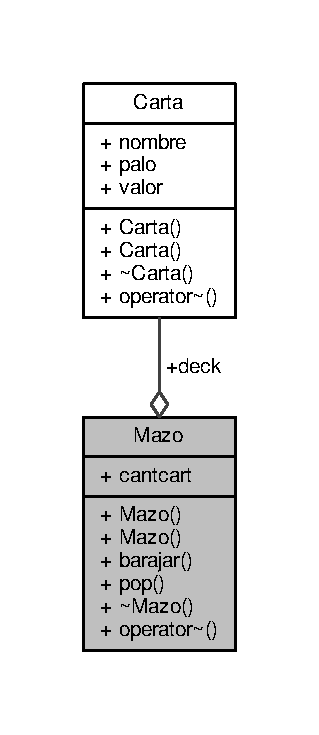
\includegraphics[width=153pt]{class_mazo__coll__graph}
\end{center}
\end{figure}
\subsection*{Public Member Functions}
\begin{DoxyCompactItemize}
\item 
\hyperlink{class_mazo_a93eaa35af9ad42840c3a37d4054ba17d}{Mazo} ()
\begin{DoxyCompactList}\small\item\em Constructor básico de clase \hyperlink{class_mazo}{Mazo}. \end{DoxyCompactList}\item 
\hyperlink{class_mazo_afa6b84ca154491f3a3258c306cffdda3}{Mazo} (string nombre, string palo, int valor)
\item 
void \hyperlink{class_mazo_ad73b15de8ae06e4e7aaecd97626bbe21}{barajar} ()
\begin{DoxyCompactList}\small\item\em Método que de forma aleatoria ordena a las cartas del objeto mazo. \end{DoxyCompactList}\item 
\hyperlink{class_carta}{Carta} \hyperlink{class_mazo_a31ede195584d6c9b6046e1a409b95540}{pop} (bool cond)
\begin{DoxyCompactList}\small\item\em Método que hace un pop al mazo, removiendo la carta que está arriba en el strack. \end{DoxyCompactList}\item 
\hyperlink{class_mazo_a2ce07ca90c706e6454ac54d727d3da2a}{$\sim$\+Mazo} ()
\begin{DoxyCompactList}\small\item\em Destructor de la clase mazo. \end{DoxyCompactList}\item 
void \hyperlink{class_mazo_a3d2974fd7edccb74895d66ccb5dc078a}{operator$\sim$} ()
\begin{DoxyCompactList}\small\item\em Método de print para la clase mazo. \end{DoxyCompactList}\end{DoxyCompactItemize}
\subsection*{Public Attributes}
\begin{DoxyCompactItemize}
\item 
\hyperlink{class_carta}{Carta} $\ast$ \hyperlink{class_mazo_a695987bdf77145b16494fa8dbd606d11}{deck}
\item 
int \hyperlink{class_mazo_af10f2aeda8faed14cbb7b0ad9febd126}{cantcart}
\end{DoxyCompactItemize}


\subsection{Constructor \& Destructor Documentation}
\hypertarget{class_mazo_a93eaa35af9ad42840c3a37d4054ba17d}{\index{Mazo@{Mazo}!Mazo@{Mazo}}
\index{Mazo@{Mazo}!Mazo@{Mazo}}
\subsubsection[{Mazo}]{\setlength{\rightskip}{0pt plus 5cm}Mazo\+::\+Mazo (
\begin{DoxyParamCaption}
{}
\end{DoxyParamCaption}
)}}\label{class_mazo_a93eaa35af9ad42840c3a37d4054ba17d}


Constructor básico de clase \hyperlink{class_mazo}{Mazo}. 

\hypertarget{class_mazo_afa6b84ca154491f3a3258c306cffdda3}{\index{Mazo@{Mazo}!Mazo@{Mazo}}
\index{Mazo@{Mazo}!Mazo@{Mazo}}
\subsubsection[{Mazo}]{\setlength{\rightskip}{0pt plus 5cm}Mazo\+::\+Mazo (
\begin{DoxyParamCaption}
\item[{string}]{nombre, }
\item[{string}]{palo, }
\item[{int}]{valor}
\end{DoxyParamCaption}
)}}\label{class_mazo_afa6b84ca154491f3a3258c306cffdda3}
\hypertarget{class_mazo_a2ce07ca90c706e6454ac54d727d3da2a}{\index{Mazo@{Mazo}!````~Mazo@{$\sim$\+Mazo}}
\index{````~Mazo@{$\sim$\+Mazo}!Mazo@{Mazo}}
\subsubsection[{$\sim$\+Mazo}]{\setlength{\rightskip}{0pt plus 5cm}Mazo\+::$\sim$\+Mazo (
\begin{DoxyParamCaption}
{}
\end{DoxyParamCaption}
)}}\label{class_mazo_a2ce07ca90c706e6454ac54d727d3da2a}


Destructor de la clase mazo. 



\subsection{Member Function Documentation}
\hypertarget{class_mazo_ad73b15de8ae06e4e7aaecd97626bbe21}{\index{Mazo@{Mazo}!barajar@{barajar}}
\index{barajar@{barajar}!Mazo@{Mazo}}
\subsubsection[{barajar}]{\setlength{\rightskip}{0pt plus 5cm}void Mazo\+::barajar (
\begin{DoxyParamCaption}
{}
\end{DoxyParamCaption}
)}}\label{class_mazo_ad73b15de8ae06e4e7aaecd97626bbe21}


Método que de forma aleatoria ordena a las cartas del objeto mazo. 



Here is the caller graph for this function\+:
\nopagebreak
\begin{figure}[H]
\begin{center}
\leavevmode
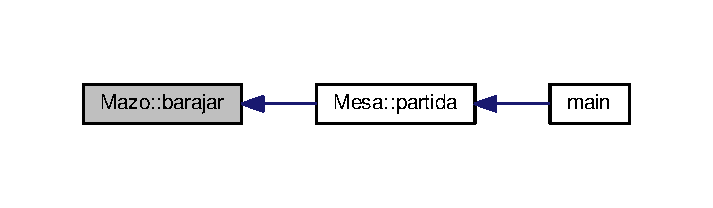
\includegraphics[width=342pt]{class_mazo_ad73b15de8ae06e4e7aaecd97626bbe21_icgraph}
\end{center}
\end{figure}


\hypertarget{class_mazo_a3d2974fd7edccb74895d66ccb5dc078a}{\index{Mazo@{Mazo}!operator````~@{operator$\sim$}}
\index{operator````~@{operator$\sim$}!Mazo@{Mazo}}
\subsubsection[{operator$\sim$}]{\setlength{\rightskip}{0pt plus 5cm}void Mazo\+::operator$\sim$ (
\begin{DoxyParamCaption}
{}
\end{DoxyParamCaption}
)}}\label{class_mazo_a3d2974fd7edccb74895d66ccb5dc078a}


Método de print para la clase mazo. 

\hypertarget{class_mazo_a31ede195584d6c9b6046e1a409b95540}{\index{Mazo@{Mazo}!pop@{pop}}
\index{pop@{pop}!Mazo@{Mazo}}
\subsubsection[{pop}]{\setlength{\rightskip}{0pt plus 5cm}{\bf Carta} Mazo\+::pop (
\begin{DoxyParamCaption}
\item[{bool}]{cond}
\end{DoxyParamCaption}
)}}\label{class_mazo_a31ede195584d6c9b6046e1a409b95540}


Método que hace un pop al mazo, removiendo la carta que está arriba en el strack. 



Here is the caller graph for this function\+:
\nopagebreak
\begin{figure}[H]
\begin{center}
\leavevmode
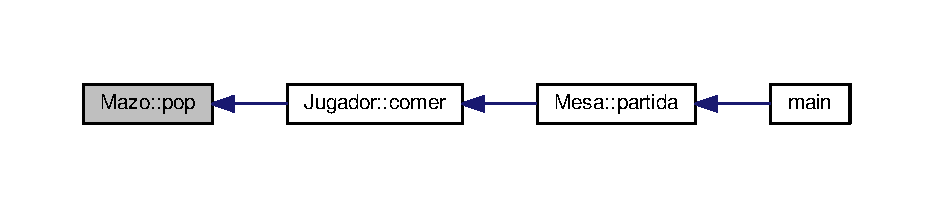
\includegraphics[width=350pt]{class_mazo_a31ede195584d6c9b6046e1a409b95540_icgraph}
\end{center}
\end{figure}




\subsection{Member Data Documentation}
\hypertarget{class_mazo_af10f2aeda8faed14cbb7b0ad9febd126}{\index{Mazo@{Mazo}!cantcart@{cantcart}}
\index{cantcart@{cantcart}!Mazo@{Mazo}}
\subsubsection[{cantcart}]{\setlength{\rightskip}{0pt plus 5cm}int Mazo\+::cantcart}}\label{class_mazo_af10f2aeda8faed14cbb7b0ad9febd126}
\hypertarget{class_mazo_a695987bdf77145b16494fa8dbd606d11}{\index{Mazo@{Mazo}!deck@{deck}}
\index{deck@{deck}!Mazo@{Mazo}}
\subsubsection[{deck}]{\setlength{\rightskip}{0pt plus 5cm}{\bf Carta}$\ast$ Mazo\+::deck}}\label{class_mazo_a695987bdf77145b16494fa8dbd606d11}


The documentation for this class was generated from the following files\+:\begin{DoxyCompactItemize}
\item 
/home/emanuel/\+Desktop/\+Labs/\+Lab\+C5/src/\hyperlink{_mazo_8h}{Mazo.\+h}\item 
/home/emanuel/\+Desktop/\+Labs/\+Lab\+C5/src/\hyperlink{_mazo_8cpp}{Mazo.\+cpp}\end{DoxyCompactItemize}

\hypertarget{class_mesa}{\section{Mesa Class Reference}
\label{class_mesa}\index{Mesa@{Mesa}}
}


{\ttfamily \#include $<$Mesa.\+h$>$}



Collaboration diagram for Mesa\+:
\nopagebreak
\begin{figure}[H]
\begin{center}
\leavevmode
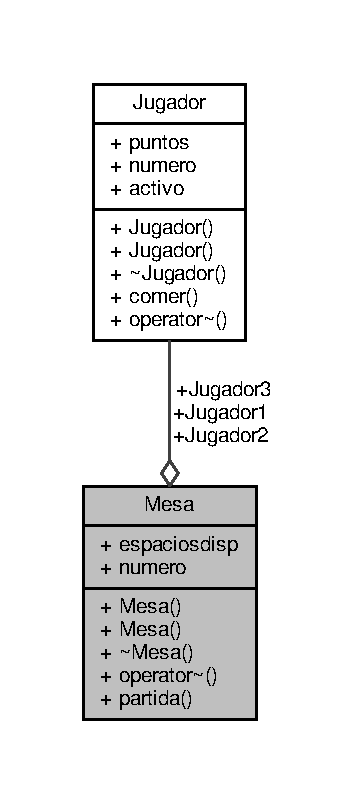
\includegraphics[width=171pt]{class_mesa__coll__graph}
\end{center}
\end{figure}
\subsection*{Public Member Functions}
\begin{DoxyCompactItemize}
\item 
\hyperlink{class_mesa_a98794038db53804cb4295480c96b2c20}{Mesa} ()
\begin{DoxyCompactList}\small\item\em Constructor básico de la clase \hyperlink{class_mesa}{Mesa}. \end{DoxyCompactList}\item 
\hyperlink{class_mesa_ac3c8674720bcb7e078272d4e95c422dc}{Mesa} (int \hyperlink{class_mesa_a704a565a0ac29cb726bb1a4e826a8127}{numero})
\begin{DoxyCompactList}\small\item\em Constructor con características de la clase \hyperlink{class_mesa}{Mesa}. \end{DoxyCompactList}\item 
\hyperlink{class_mesa_aa0a1b83b8058f80f4f27ec46cc5e9524}{$\sim$\+Mesa} ()
\begin{DoxyCompactList}\small\item\em Destructor de la clase \hyperlink{class_mesa}{Mesa}. \end{DoxyCompactList}\item 
void \hyperlink{class_mesa_aad6dc6e5101774e4caad60b01c9225b1}{operator$\sim$} ()
\begin{DoxyCompactList}\small\item\em Método de print para objetos \hyperlink{class_mesa}{Mesa}. \end{DoxyCompactList}\item 
void \hyperlink{class_mesa_a3b925c89a9f8ec6f1b43bbf70c76bb5d}{partida} (\hyperlink{class_fila}{Fila} \&fila)
\begin{DoxyCompactList}\small\item\em Método en el cuál 1, 2 o 3 jugadores juegan una partida de blackjack. \end{DoxyCompactList}\end{DoxyCompactItemize}
\subsection*{Public Attributes}
\begin{DoxyCompactItemize}
\item 
int \hyperlink{class_mesa_ab5d554a7073ea0a71f19bb796f43ec83}{espaciosdisp}
\item 
int \hyperlink{class_mesa_a704a565a0ac29cb726bb1a4e826a8127}{numero}
\item 
\hyperlink{class_jugador}{Jugador} \hyperlink{class_mesa_a31db9c4417611b8e6eb2b8695174775d}{Jugador1}
\item 
\hyperlink{class_jugador}{Jugador} \hyperlink{class_mesa_af43fd0e2946bb98c12551a83bff12885}{Jugador2}
\item 
\hyperlink{class_jugador}{Jugador} \hyperlink{class_mesa_a522e14a1213755c443bd3e00da072a11}{Jugador3}
\end{DoxyCompactItemize}


\subsection{Constructor \& Destructor Documentation}
\hypertarget{class_mesa_a98794038db53804cb4295480c96b2c20}{\index{Mesa@{Mesa}!Mesa@{Mesa}}
\index{Mesa@{Mesa}!Mesa@{Mesa}}
\subsubsection[{Mesa}]{\setlength{\rightskip}{0pt plus 5cm}Mesa\+::\+Mesa (
\begin{DoxyParamCaption}
{}
\end{DoxyParamCaption}
)}}\label{class_mesa_a98794038db53804cb4295480c96b2c20}


Constructor básico de la clase \hyperlink{class_mesa}{Mesa}. 

\hypertarget{class_mesa_ac3c8674720bcb7e078272d4e95c422dc}{\index{Mesa@{Mesa}!Mesa@{Mesa}}
\index{Mesa@{Mesa}!Mesa@{Mesa}}
\subsubsection[{Mesa}]{\setlength{\rightskip}{0pt plus 5cm}Mesa\+::\+Mesa (
\begin{DoxyParamCaption}
\item[{int}]{numero}
\end{DoxyParamCaption}
)}}\label{class_mesa_ac3c8674720bcb7e078272d4e95c422dc}


Constructor con características de la clase \hyperlink{class_mesa}{Mesa}. 

\hypertarget{class_mesa_aa0a1b83b8058f80f4f27ec46cc5e9524}{\index{Mesa@{Mesa}!````~Mesa@{$\sim$\+Mesa}}
\index{````~Mesa@{$\sim$\+Mesa}!Mesa@{Mesa}}
\subsubsection[{$\sim$\+Mesa}]{\setlength{\rightskip}{0pt plus 5cm}Mesa\+::$\sim$\+Mesa (
\begin{DoxyParamCaption}
{}
\end{DoxyParamCaption}
)}}\label{class_mesa_aa0a1b83b8058f80f4f27ec46cc5e9524}


Destructor de la clase \hyperlink{class_mesa}{Mesa}. 



\subsection{Member Function Documentation}
\hypertarget{class_mesa_aad6dc6e5101774e4caad60b01c9225b1}{\index{Mesa@{Mesa}!operator````~@{operator$\sim$}}
\index{operator````~@{operator$\sim$}!Mesa@{Mesa}}
\subsubsection[{operator$\sim$}]{\setlength{\rightskip}{0pt plus 5cm}void Mesa\+::operator$\sim$ (
\begin{DoxyParamCaption}
{}
\end{DoxyParamCaption}
)}}\label{class_mesa_aad6dc6e5101774e4caad60b01c9225b1}


Método de print para objetos \hyperlink{class_mesa}{Mesa}. 

\hypertarget{class_mesa_a3b925c89a9f8ec6f1b43bbf70c76bb5d}{\index{Mesa@{Mesa}!partida@{partida}}
\index{partida@{partida}!Mesa@{Mesa}}
\subsubsection[{partida}]{\setlength{\rightskip}{0pt plus 5cm}void Mesa\+::partida (
\begin{DoxyParamCaption}
\item[{{\bf Fila} \&}]{fila}
\end{DoxyParamCaption}
)}}\label{class_mesa_a3b925c89a9f8ec6f1b43bbf70c76bb5d}


Método en el cuál 1, 2 o 3 jugadores juegan una partida de blackjack. 



Here is the call graph for this function\+:
\nopagebreak
\begin{figure}[H]
\begin{center}
\leavevmode
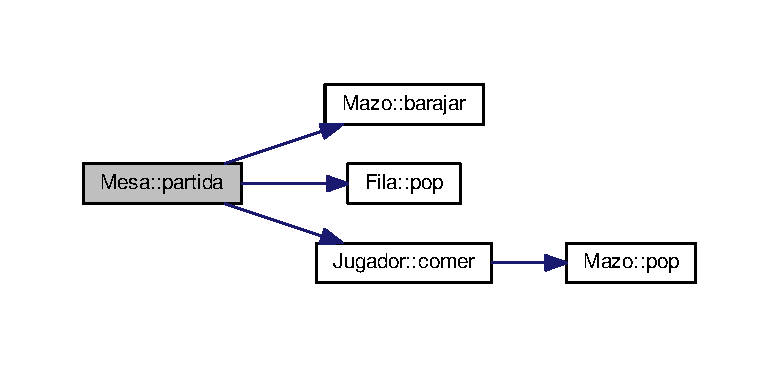
\includegraphics[width=350pt]{class_mesa_a3b925c89a9f8ec6f1b43bbf70c76bb5d_cgraph}
\end{center}
\end{figure}




Here is the caller graph for this function\+:
\nopagebreak
\begin{figure}[H]
\begin{center}
\leavevmode
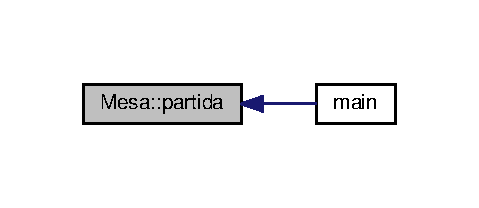
\includegraphics[width=230pt]{class_mesa_a3b925c89a9f8ec6f1b43bbf70c76bb5d_icgraph}
\end{center}
\end{figure}




\subsection{Member Data Documentation}
\hypertarget{class_mesa_ab5d554a7073ea0a71f19bb796f43ec83}{\index{Mesa@{Mesa}!espaciosdisp@{espaciosdisp}}
\index{espaciosdisp@{espaciosdisp}!Mesa@{Mesa}}
\subsubsection[{espaciosdisp}]{\setlength{\rightskip}{0pt plus 5cm}int Mesa\+::espaciosdisp}}\label{class_mesa_ab5d554a7073ea0a71f19bb796f43ec83}
\hypertarget{class_mesa_a31db9c4417611b8e6eb2b8695174775d}{\index{Mesa@{Mesa}!Jugador1@{Jugador1}}
\index{Jugador1@{Jugador1}!Mesa@{Mesa}}
\subsubsection[{Jugador1}]{\setlength{\rightskip}{0pt plus 5cm}{\bf Jugador} Mesa\+::\+Jugador1}}\label{class_mesa_a31db9c4417611b8e6eb2b8695174775d}
\hypertarget{class_mesa_af43fd0e2946bb98c12551a83bff12885}{\index{Mesa@{Mesa}!Jugador2@{Jugador2}}
\index{Jugador2@{Jugador2}!Mesa@{Mesa}}
\subsubsection[{Jugador2}]{\setlength{\rightskip}{0pt plus 5cm}{\bf Jugador} Mesa\+::\+Jugador2}}\label{class_mesa_af43fd0e2946bb98c12551a83bff12885}
\hypertarget{class_mesa_a522e14a1213755c443bd3e00da072a11}{\index{Mesa@{Mesa}!Jugador3@{Jugador3}}
\index{Jugador3@{Jugador3}!Mesa@{Mesa}}
\subsubsection[{Jugador3}]{\setlength{\rightskip}{0pt plus 5cm}{\bf Jugador} Mesa\+::\+Jugador3}}\label{class_mesa_a522e14a1213755c443bd3e00da072a11}
\hypertarget{class_mesa_a704a565a0ac29cb726bb1a4e826a8127}{\index{Mesa@{Mesa}!numero@{numero}}
\index{numero@{numero}!Mesa@{Mesa}}
\subsubsection[{numero}]{\setlength{\rightskip}{0pt plus 5cm}int Mesa\+::numero}}\label{class_mesa_a704a565a0ac29cb726bb1a4e826a8127}


The documentation for this class was generated from the following files\+:\begin{DoxyCompactItemize}
\item 
/home/emanuel/\+Desktop/\+Labs/\+Lab\+C5/src/\hyperlink{_mesa_8h}{Mesa.\+h}\item 
/home/emanuel/\+Desktop/\+Labs/\+Lab\+C5/src/\hyperlink{_mesa_8cpp}{Mesa.\+cpp}\end{DoxyCompactItemize}

\chapter{File Documentation}
\hypertarget{_carta_8cpp}{\section{/home/emanuel/\+Desktop/\+Labs/\+Lab\+C5/src/\+Carta.cpp File Reference}
\label{_carta_8cpp}\index{/home/emanuel/\+Desktop/\+Labs/\+Lab\+C5/src/\+Carta.\+cpp@{/home/emanuel/\+Desktop/\+Labs/\+Lab\+C5/src/\+Carta.\+cpp}}
}
{\ttfamily \#include \char`\"{}Carta.\+h\char`\"{}}\\*
{\ttfamily \#include $<$iostream$>$}\\*
{\ttfamily \#include \char`\"{}string\char`\"{}}\\*
Include dependency graph for Carta.\+cpp\+:
\nopagebreak
\begin{figure}[H]
\begin{center}
\leavevmode
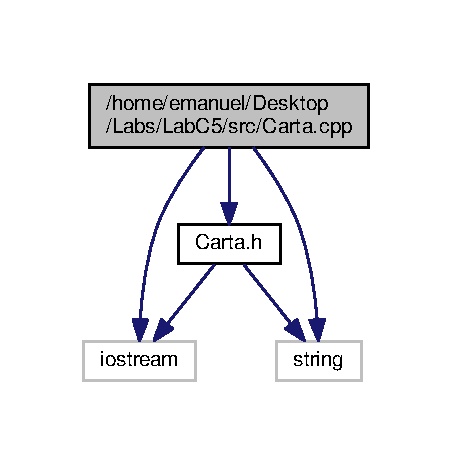
\includegraphics[width=217pt]{_carta_8cpp__incl}
\end{center}
\end{figure}

\hypertarget{_carta_8h}{\section{/home/emanuel/\+Desktop/\+Labs/\+Lab\+C5/src/\+Carta.h File Reference}
\label{_carta_8h}\index{/home/emanuel/\+Desktop/\+Labs/\+Lab\+C5/src/\+Carta.\+h@{/home/emanuel/\+Desktop/\+Labs/\+Lab\+C5/src/\+Carta.\+h}}
}
{\ttfamily \#include $<$iostream$>$}\\*
{\ttfamily \#include \char`\"{}string\char`\"{}}\\*
Include dependency graph for Carta.\+h\+:
\nopagebreak
\begin{figure}[H]
\begin{center}
\leavevmode
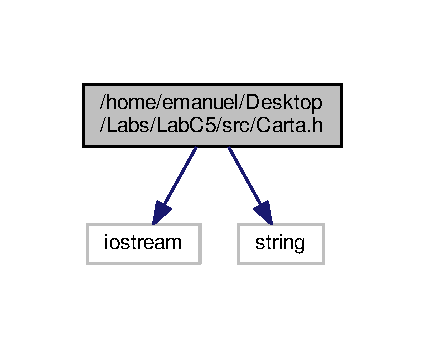
\includegraphics[width=204pt]{_carta_8h__incl}
\end{center}
\end{figure}
This graph shows which files directly or indirectly include this file\+:
\nopagebreak
\begin{figure}[H]
\begin{center}
\leavevmode
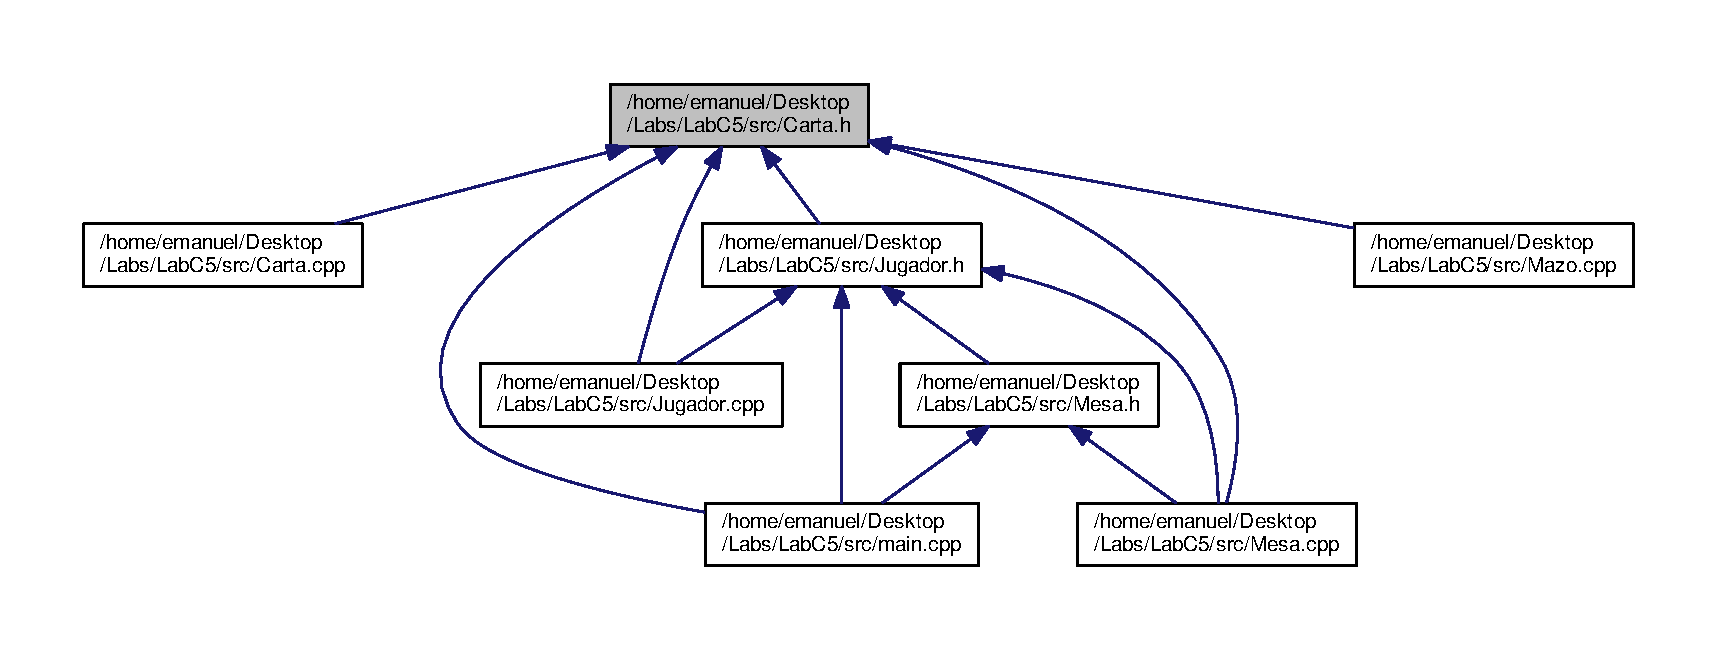
\includegraphics[width=350pt]{_carta_8h__dep__incl}
\end{center}
\end{figure}
\subsection*{Classes}
\begin{DoxyCompactItemize}
\item 
class \hyperlink{class_carta}{Carta}
\end{DoxyCompactItemize}

\hypertarget{_fila_8cpp}{\section{/home/emanuel/\+Desktop/\+Labs/\+Lab\+C5/src/\+Fila.cpp File Reference}
\label{_fila_8cpp}\index{/home/emanuel/\+Desktop/\+Labs/\+Lab\+C5/src/\+Fila.\+cpp@{/home/emanuel/\+Desktop/\+Labs/\+Lab\+C5/src/\+Fila.\+cpp}}
}
{\ttfamily \#include \char`\"{}Fila.\+h\char`\"{}}\\*
{\ttfamily \#include $<$iostream$>$}\\*
{\ttfamily \#include \char`\"{}string\char`\"{}}\\*
Include dependency graph for Fila.\+cpp\+:
\nopagebreak
\begin{figure}[H]
\begin{center}
\leavevmode
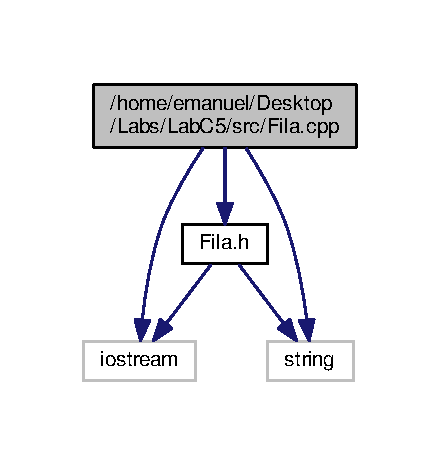
\includegraphics[width=211pt]{_fila_8cpp__incl}
\end{center}
\end{figure}

\hypertarget{_fila_8h}{\section{/home/emanuel/\+Desktop/\+Labs/\+Lab\+C5/src/\+Fila.h File Reference}
\label{_fila_8h}\index{/home/emanuel/\+Desktop/\+Labs/\+Lab\+C5/src/\+Fila.\+h@{/home/emanuel/\+Desktop/\+Labs/\+Lab\+C5/src/\+Fila.\+h}}
}
{\ttfamily \#include $<$iostream$>$}\\*
{\ttfamily \#include \char`\"{}string\char`\"{}}\\*
Include dependency graph for Fila.\+h\+:
\nopagebreak
\begin{figure}[H]
\begin{center}
\leavevmode
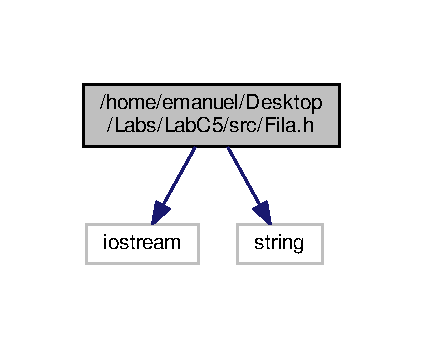
\includegraphics[width=203pt]{_fila_8h__incl}
\end{center}
\end{figure}
This graph shows which files directly or indirectly include this file\+:
\nopagebreak
\begin{figure}[H]
\begin{center}
\leavevmode
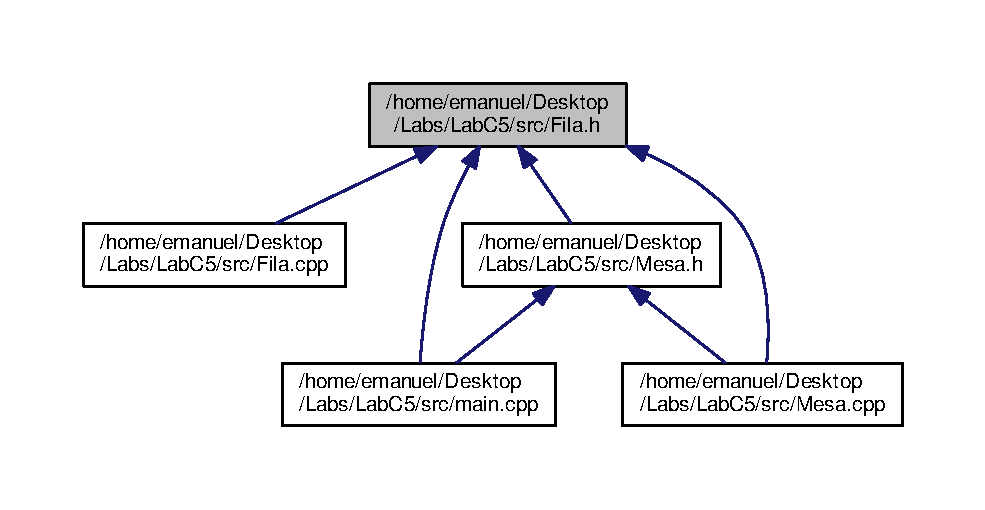
\includegraphics[width=350pt]{_fila_8h__dep__incl}
\end{center}
\end{figure}
\subsection*{Classes}
\begin{DoxyCompactItemize}
\item 
class \hyperlink{class_fila}{Fila}
\end{DoxyCompactItemize}

\hypertarget{_jugador_8cpp}{\section{/home/emanuel/\+Desktop/\+Labs/\+Lab\+C5/src/\+Jugador.cpp File Reference}
\label{_jugador_8cpp}\index{/home/emanuel/\+Desktop/\+Labs/\+Lab\+C5/src/\+Jugador.\+cpp@{/home/emanuel/\+Desktop/\+Labs/\+Lab\+C5/src/\+Jugador.\+cpp}}
}
{\ttfamily \#include \char`\"{}Jugador.\+h\char`\"{}}\\*
{\ttfamily \#include $<$iostream$>$}\\*
{\ttfamily \#include \char`\"{}string\char`\"{}}\\*
{\ttfamily \#include \char`\"{}Carta.\+h\char`\"{}}\\*
{\ttfamily \#include \char`\"{}Mazo.\+h\char`\"{}}\\*
Include dependency graph for Jugador.\+cpp\+:
\nopagebreak
\begin{figure}[H]
\begin{center}
\leavevmode
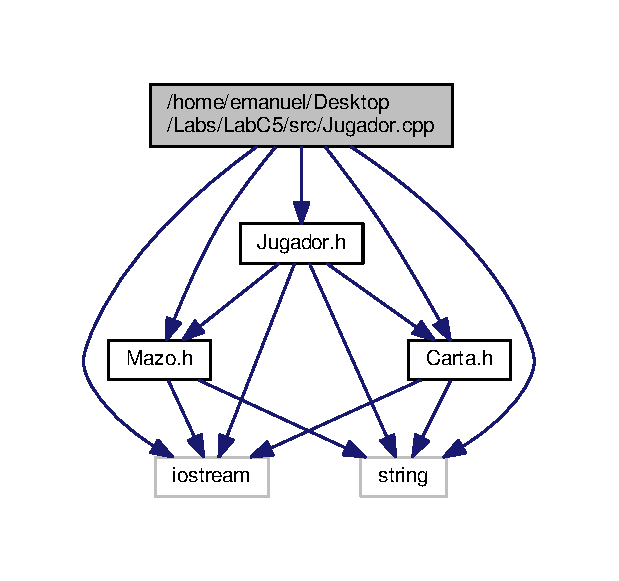
\includegraphics[width=297pt]{_jugador_8cpp__incl}
\end{center}
\end{figure}

\hypertarget{_jugador_8h}{\section{/home/emanuel/\+Desktop/\+Labs/\+Lab\+C5/src/\+Jugador.h File Reference}
\label{_jugador_8h}\index{/home/emanuel/\+Desktop/\+Labs/\+Lab\+C5/src/\+Jugador.\+h@{/home/emanuel/\+Desktop/\+Labs/\+Lab\+C5/src/\+Jugador.\+h}}
}
{\ttfamily \#include $<$iostream$>$}\\*
{\ttfamily \#include \char`\"{}string\char`\"{}}\\*
{\ttfamily \#include \char`\"{}Carta.\+h\char`\"{}}\\*
{\ttfamily \#include \char`\"{}Mazo.\+h\char`\"{}}\\*
Include dependency graph for Jugador.\+h\+:
\nopagebreak
\begin{figure}[H]
\begin{center}
\leavevmode
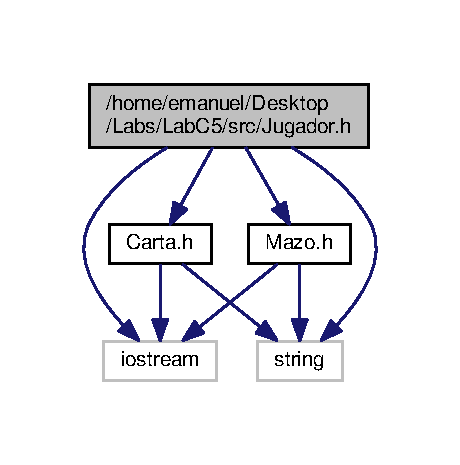
\includegraphics[width=221pt]{_jugador_8h__incl}
\end{center}
\end{figure}
This graph shows which files directly or indirectly include this file\+:
\nopagebreak
\begin{figure}[H]
\begin{center}
\leavevmode
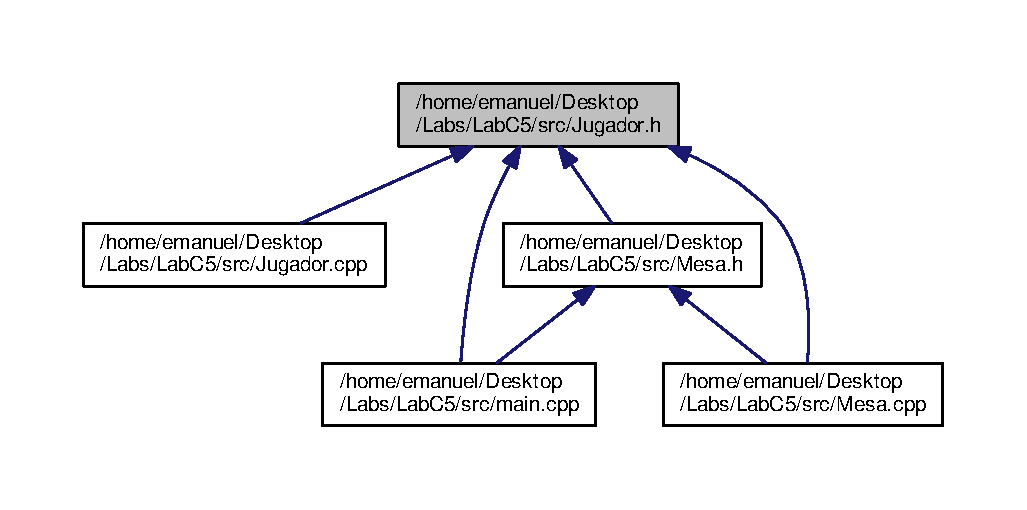
\includegraphics[width=350pt]{_jugador_8h__dep__incl}
\end{center}
\end{figure}
\subsection*{Classes}
\begin{DoxyCompactItemize}
\item 
class \hyperlink{class_jugador}{Jugador}
\end{DoxyCompactItemize}

\hypertarget{main_8cpp}{\section{main.\+cpp File Reference}
\label{main_8cpp}\index{main.\+cpp@{main.\+cpp}}
}
{\ttfamily \#include $<$cstdlib$>$}\\*
{\ttfamily \#include \char`\"{}Node.\+h\char`\"{}}\\*
{\ttfamily \#include \char`\"{}Graph.\+h\char`\"{}}\\*
{\ttfamily \#include $<$queue$>$}\\*
Include dependency graph for main.\+cpp\+:\nopagebreak
\begin{figure}[H]
\begin{center}
\leavevmode
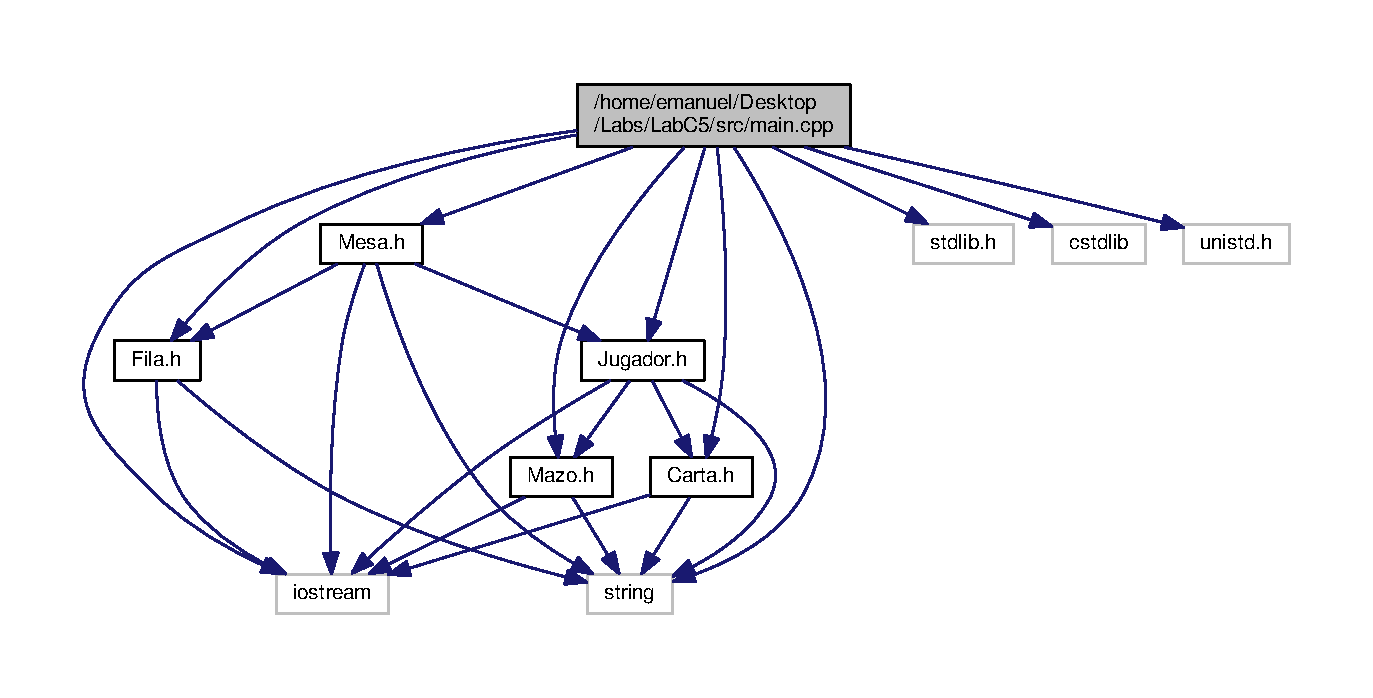
\includegraphics[width=350pt]{main_8cpp__incl}
\end{center}
\end{figure}
\subsection*{Macros}
\begin{DoxyCompactItemize}
\item 
\#define \hyperlink{main_8cpp_a4fc34b120ed3bd1120c1eb36abbcd6af}{N\+L}~cout $<$$<$ endl;
\item 
\#define \hyperlink{main_8cpp_aecd69d9a67487cc45c38eb184c50538a}{S\+P}~\char`\"{} \char`\"{}
\end{DoxyCompactItemize}
\subsection*{Functions}
\begin{DoxyCompactItemize}
\item 
int \hyperlink{main_8cpp_a3c04138a5bfe5d72780bb7e82a18e627}{main} (int argc, char $\ast$$\ast$argv)
\end{DoxyCompactItemize}


\subsection{Macro Definition Documentation}
\hypertarget{main_8cpp_a4fc34b120ed3bd1120c1eb36abbcd6af}{\index{main.\+cpp@{main.\+cpp}!N\+L@{N\+L}}
\index{N\+L@{N\+L}!main.\+cpp@{main.\+cpp}}
\subsubsection[{N\+L}]{\setlength{\rightskip}{0pt plus 5cm}\#define N\+L~cout $<$$<$ endl;}}\label{main_8cpp_a4fc34b120ed3bd1120c1eb36abbcd6af}
\hypertarget{main_8cpp_aecd69d9a67487cc45c38eb184c50538a}{\index{main.\+cpp@{main.\+cpp}!S\+P@{S\+P}}
\index{S\+P@{S\+P}!main.\+cpp@{main.\+cpp}}
\subsubsection[{S\+P}]{\setlength{\rightskip}{0pt plus 5cm}\#define S\+P~\char`\"{} \char`\"{}}}\label{main_8cpp_aecd69d9a67487cc45c38eb184c50538a}


\subsection{Function Documentation}
\hypertarget{main_8cpp_a3c04138a5bfe5d72780bb7e82a18e627}{\index{main.\+cpp@{main.\+cpp}!main@{main}}
\index{main@{main}!main.\+cpp@{main.\+cpp}}
\subsubsection[{main}]{\setlength{\rightskip}{0pt plus 5cm}int main (
\begin{DoxyParamCaption}
\item[{int}]{argc, }
\item[{char $\ast$$\ast$}]{argv}
\end{DoxyParamCaption}
)}}\label{main_8cpp_a3c04138a5bfe5d72780bb7e82a18e627}


Here is the call graph for this function\+:\nopagebreak
\begin{figure}[H]
\begin{center}
\leavevmode
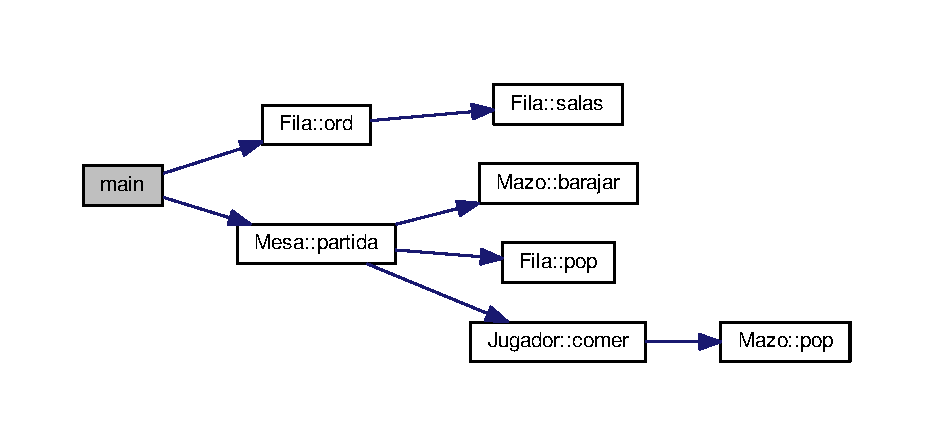
\includegraphics[width=240pt]{main_8cpp_a3c04138a5bfe5d72780bb7e82a18e627_cgraph}
\end{center}
\end{figure}



\hypertarget{_mazo_8cpp}{\section{/home/emanuel/\+Desktop/\+Labs/\+Lab\+C5/src/\+Mazo.cpp File Reference}
\label{_mazo_8cpp}\index{/home/emanuel/\+Desktop/\+Labs/\+Lab\+C5/src/\+Mazo.\+cpp@{/home/emanuel/\+Desktop/\+Labs/\+Lab\+C5/src/\+Mazo.\+cpp}}
}
{\ttfamily \#include \char`\"{}Carta.\+h\char`\"{}}\\*
{\ttfamily \#include $<$iostream$>$}\\*
{\ttfamily \#include \char`\"{}string\char`\"{}}\\*
{\ttfamily \#include \char`\"{}Mazo.\+h\char`\"{}}\\*
{\ttfamily \#include $<$cstdlib$>$}\\*
{\ttfamily \#include \char`\"{}time.\+h\char`\"{}}\\*
Include dependency graph for Mazo.\+cpp\+:
\nopagebreak
\begin{figure}[H]
\begin{center}
\leavevmode
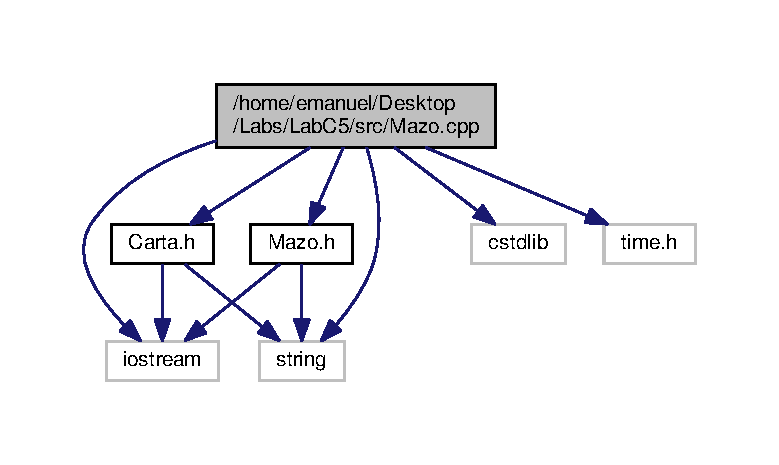
\includegraphics[width=350pt]{_mazo_8cpp__incl}
\end{center}
\end{figure}

\hypertarget{_mazo_8h}{\section{/home/emanuel/\+Desktop/\+Labs/\+Lab\+C5/src/\+Mazo.h File Reference}
\label{_mazo_8h}\index{/home/emanuel/\+Desktop/\+Labs/\+Lab\+C5/src/\+Mazo.\+h@{/home/emanuel/\+Desktop/\+Labs/\+Lab\+C5/src/\+Mazo.\+h}}
}
{\ttfamily \#include $<$iostream$>$}\\*
{\ttfamily \#include \char`\"{}string\char`\"{}}\\*
Include dependency graph for Mazo.\+h\+:
\nopagebreak
\begin{figure}[H]
\begin{center}
\leavevmode
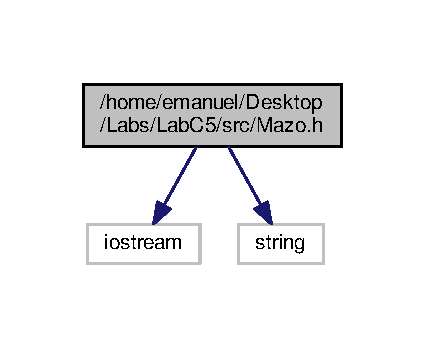
\includegraphics[width=204pt]{_mazo_8h__incl}
\end{center}
\end{figure}
This graph shows which files directly or indirectly include this file\+:
\nopagebreak
\begin{figure}[H]
\begin{center}
\leavevmode
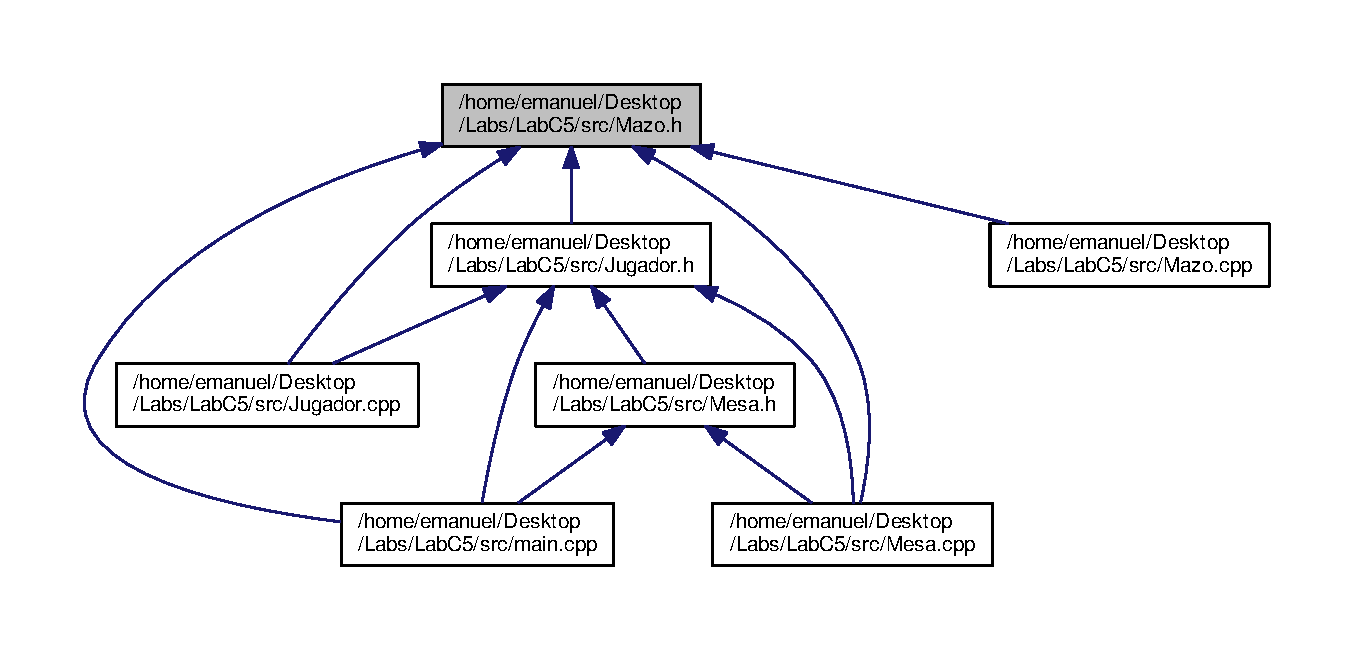
\includegraphics[width=350pt]{_mazo_8h__dep__incl}
\end{center}
\end{figure}
\subsection*{Classes}
\begin{DoxyCompactItemize}
\item 
class \hyperlink{class_mazo}{Mazo}
\end{DoxyCompactItemize}

\hypertarget{_mesa_8cpp}{\section{/home/emanuel/\+Desktop/\+Labs/\+Lab\+C5/src/\+Mesa.cpp File Reference}
\label{_mesa_8cpp}\index{/home/emanuel/\+Desktop/\+Labs/\+Lab\+C5/src/\+Mesa.\+cpp@{/home/emanuel/\+Desktop/\+Labs/\+Lab\+C5/src/\+Mesa.\+cpp}}
}
{\ttfamily \#include \char`\"{}Mesa.\+h\char`\"{}}\\*
{\ttfamily \#include $<$iostream$>$}\\*
{\ttfamily \#include \char`\"{}string\char`\"{}}\\*
{\ttfamily \#include \char`\"{}Carta.\+h\char`\"{}}\\*
{\ttfamily \#include \char`\"{}Mazo.\+h\char`\"{}}\\*
{\ttfamily \#include \char`\"{}Jugador.\+h\char`\"{}}\\*
{\ttfamily \#include \char`\"{}Fila.\+h\char`\"{}}\\*
Include dependency graph for Mesa.\+cpp\+:
\nopagebreak
\begin{figure}[H]
\begin{center}
\leavevmode
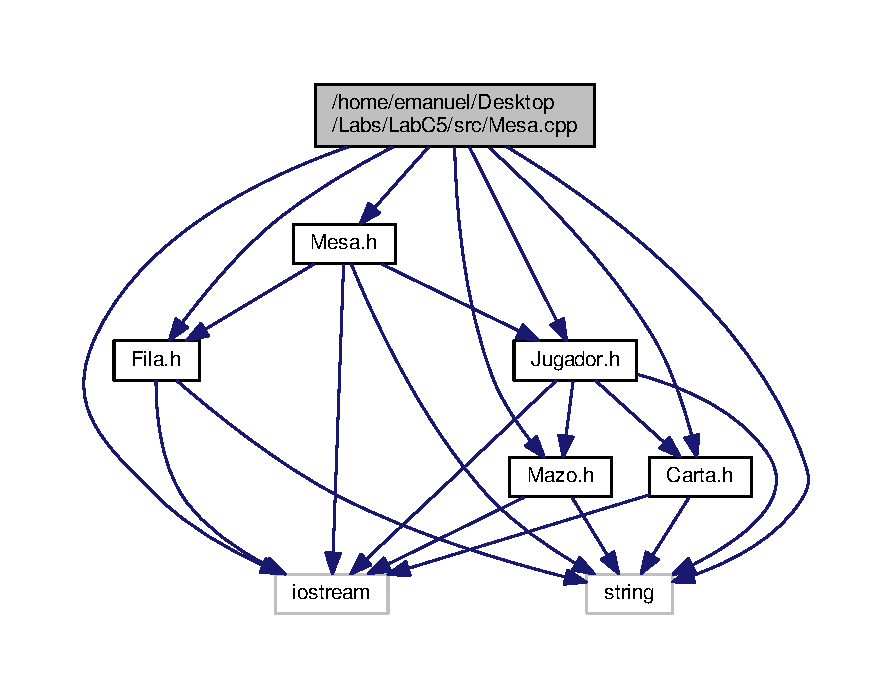
\includegraphics[width=350pt]{_mesa_8cpp__incl}
\end{center}
\end{figure}

\hypertarget{_mesa_8h}{\section{/home/emanuel/\+Desktop/\+Labs/\+Lab\+C5/src/\+Mesa.h File Reference}
\label{_mesa_8h}\index{/home/emanuel/\+Desktop/\+Labs/\+Lab\+C5/src/\+Mesa.\+h@{/home/emanuel/\+Desktop/\+Labs/\+Lab\+C5/src/\+Mesa.\+h}}
}
{\ttfamily \#include $<$iostream$>$}\\*
{\ttfamily \#include \char`\"{}string\char`\"{}}\\*
{\ttfamily \#include \char`\"{}Jugador.\+h\char`\"{}}\\*
{\ttfamily \#include \char`\"{}Fila.\+h\char`\"{}}\\*
Include dependency graph for Mesa.\+h\+:
\nopagebreak
\begin{figure}[H]
\begin{center}
\leavevmode
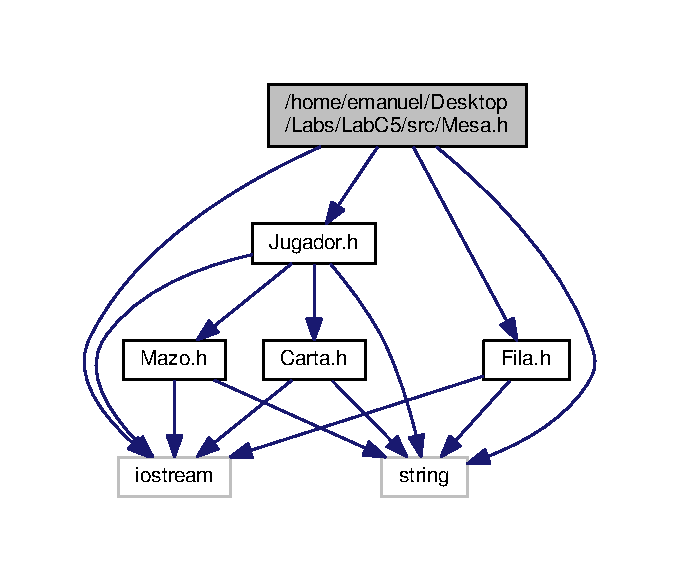
\includegraphics[width=326pt]{_mesa_8h__incl}
\end{center}
\end{figure}
This graph shows which files directly or indirectly include this file\+:
\nopagebreak
\begin{figure}[H]
\begin{center}
\leavevmode
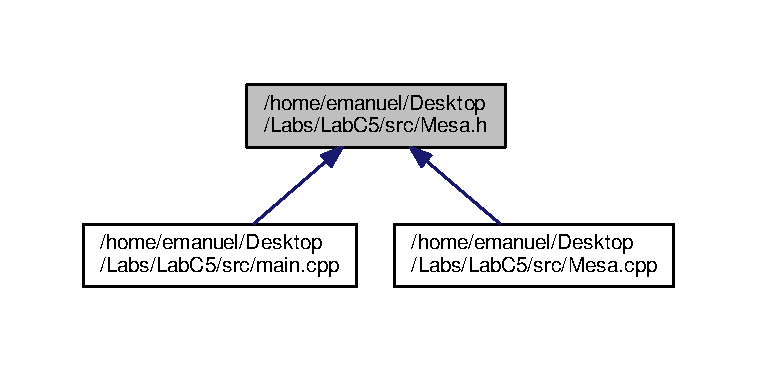
\includegraphics[width=350pt]{_mesa_8h__dep__incl}
\end{center}
\end{figure}
\subsection*{Classes}
\begin{DoxyCompactItemize}
\item 
class \hyperlink{class_mesa}{Mesa}
\end{DoxyCompactItemize}

%--- End generated contents ---

% Index
\newpage
\phantomsection
\addcontentsline{toc}{chapter}{Index}
\printindex

\end{document}
